\subsection{Overview}

\hspace{\parindent}In this section the whole process and the idea of the system implementation is explained in detail. The whole integration and implementation process of the already presented subcomponents of the system,  together with the testing plan is a very detailed and specific process. In order to get the best possible picture of the recommended implementation process, both diagrams and detailed explanations are used. \newline

As mentioned in the \hyperlink{section.2}{second section}, the system is divided into three layers: presentation layer, application layer, and data layer. Each of these layers holds one major subcomponent; Phone app, Application server, and Database, respectively.  \newline

 

These subcomponents feature many different services, managers, and interfaces, which can be found in the \hyperlink{section.2}{second section} as well. Detailed implementation of those is available only for the Application server subcomponent since most of the application logic is happening there. \newline

 

Google Maps API and Database are external and somewhat outside of our control, which also has to be taken into account during the integration and testing process.  


\subsubsection{Importance of features}

\begin{table}[H]
\begin{flushleft}
\begin{tabular}{|l|l|l|}
\hline
\textbf{Function }& \textbf{Level of importance} & \textbf{Implementation difficulty} \\
\hline
Login & Users – Low; Stores - High & Low \\
\hline
Requesting a ticket & High & Medium \\
\hline
Booking a visit & Low & High \\
\hline
Locating services & Low & Medium \\
\hline
Estimated time calculation & Low & Medium \\
\hline
Store selection & High & Low  \\
\hline
\end{tabular}
\end{flushleft}
\caption{\textbf{Importance of features}}
\label{tab:feat1}
\end{table}

\newpage

\subsection{Implementation}
\hspace{\parindent}The desired implementation process technique for this project is top-down. Since all major system components are already known and the application has a clear cut of what it should exactly do, we believe this is the way to go. By using this design technique, most of the biggest components are implemented and defined at the beginning and we work our way down to the smaller ones. This gives us a clear picture of the whole system and strong points to lean on when implementing smaller parts. The opposite technique bottom-up, which is used to build the system from the ground up, defining smaller components and then searching for the bigger picture, would be slower to implement and unnecessary since the main goals and components are clearly defined. \newline

The order of developing and integrating major components of the system should be the following:

First we develop a basic app and set up a database – this way we already have a basic system and can work on connecting it with an application server for basic functions. 

The setup of the application server and application logic follows. 

Director, RequestManager, and DB service should follow, creating a set of the most important subcomponents that allow the app to communicate with Database. Smaller parts of these components, like QueueManager, TicketManager, and others are to be implemented at the end. 

At the end, other smaller components, like StoreSelectionManager, StoreManager and LoginManager are implemented, to extend the functionalities of the application. After that other components of the RequestManager come in line. 

Finally, GoogleMapsService can be implemented at the end since it is used the least and is the least important part of the system.  \newline

 

This design flow will allow for easier testing of the major components. Testing interconnection and communication within the components will be of key to develop a reliable system. Once that is set up, smaller functionalities of the system can be implemented and tested, with the focus staying on the bigger and more important functions. That way the system can even go through some sort of a beta phase testing with the most important functionalities being set up properly and having the customers test them out. Even if some components are not tested and set up then, the app can go into circulation with more important functions working, allowing further development to not slow down the release of the app. \newpage

\subsection{Integration strategy}

\hspace{\parindent}Using the following components, the strategy regarding integration order explained in the previous section is showcased. Each component is implemented one-by-one or in groups of up to three subcomponents. This policy allows fastest development, while still maintaining a coherent global picture in mind. 

 
After PhoneApp and Database have been set up, the ApplicationServer is being implemented. 

 
\begin{figure}[!h]
\centering
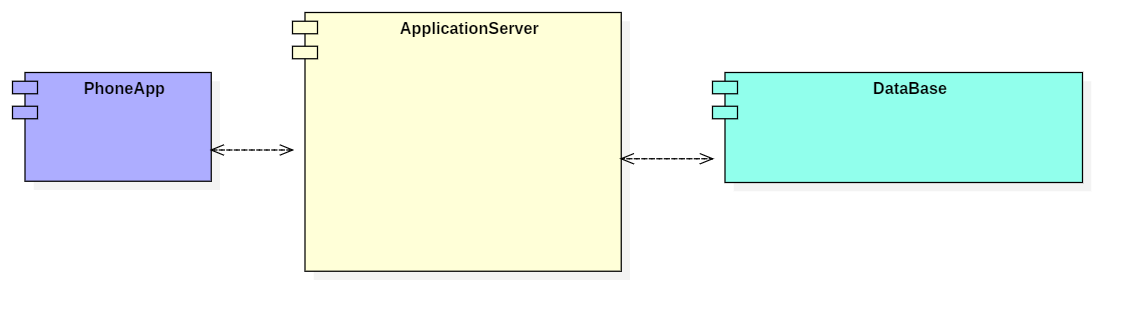
\includegraphics[width=\textwidth]{Images/IntegrationDiagram1}
\caption{\label{fig:imp1}\textbf{Integration diagram 1}}
\end{figure}
 

Director and DBService come first – ensuring that the connection and communication is properly implemented between PhoneApp and Database. Setting the director up is the most important step – with proper basic implementation, all of the other components and services are going to be to easily implemented and connected to Director.  

 

\begin{figure}[!h]
\centering
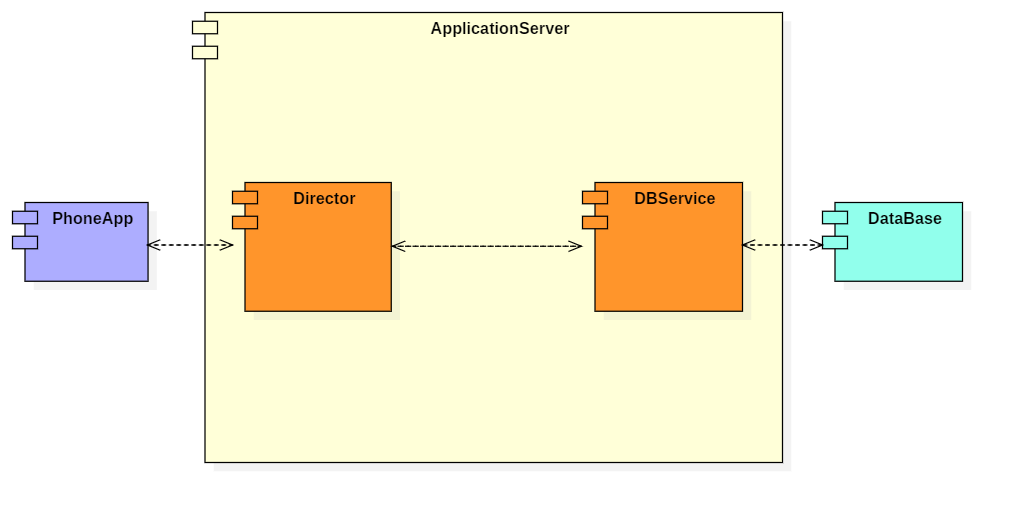
\includegraphics[width=\textwidth]{Images/IntegrationDiagram2}
\caption{\label{fig:imp2}\textbf{Integration diagram 2}}
\end{figure}

 

Request manager is the third subcomponent to be implemented, being connected both to Director and DBService. Most of the requests will go through RequestManager before heading to DBService, rather than going directly through Director, because some additional computation has to be done via the services located in RequestManager. 

 
\begin{figure}[!h]
\centering
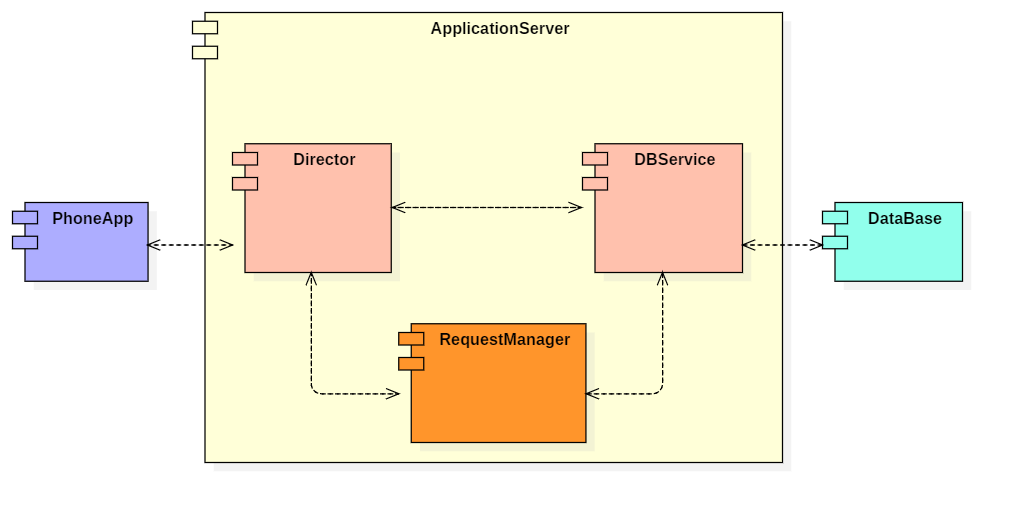
\includegraphics[width=\textwidth]{Images/IntegrationDiagram3}
\caption{\label{fig:imp3}\textbf{Integration diagram 3}}
\end{figure}

 

Managers regarding store selection and store manager login are implemented. This brings in another part of the app into existence, with all of the other components implemented so far being user oriented, while this one is admin oriented. With this, the store manager connection and login to the store can be tested. 

 
\begin{figure}[!h]
\centering
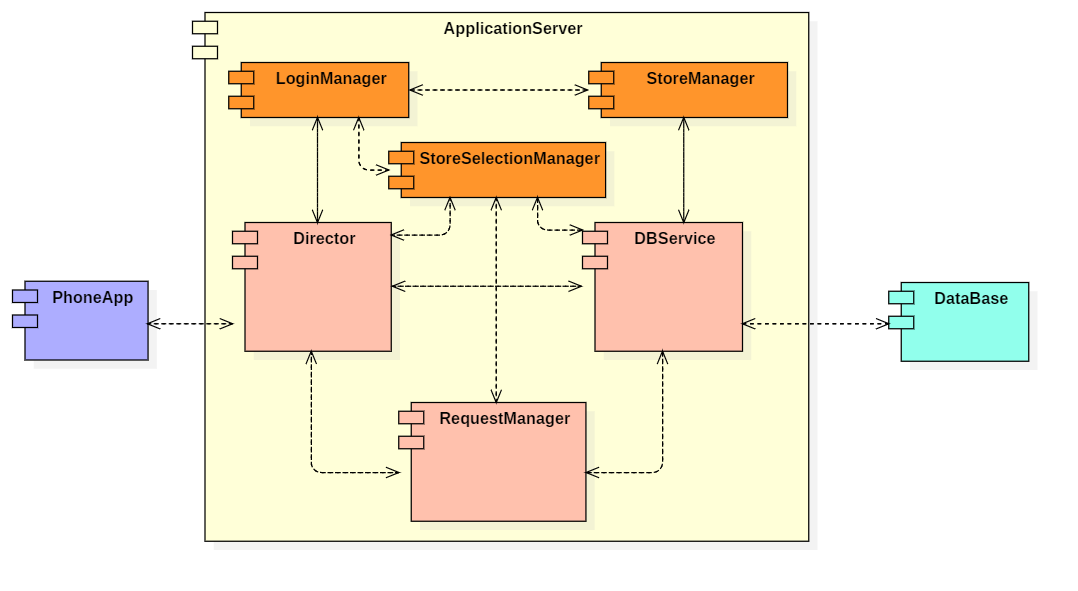
\includegraphics[width=\textwidth]{Images/IntegrationDiagram4}
\caption{\label{fig:imp4}\textbf{Integration diagram 4}}
\end{figure}
 

Lastly, all of the services in StoreManager and RequestManager are implemented. Now the ticket and queue handling are available, controlling influx of people to the store, and other functionalities like "Book a visit" are available. After all of these services have been set up and properly interconnected, GoogleMapsService can be implemented to finalize the system.

\begin{figure}[!h]
\centering
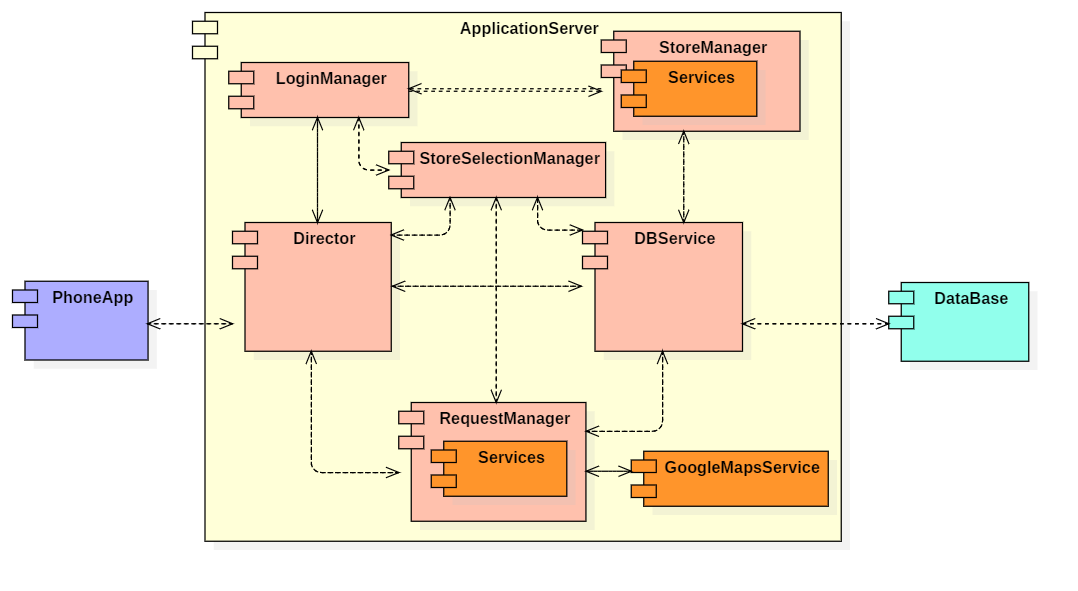
\includegraphics[width=\textwidth]{Images/IntegrationDiagram5}
\caption{\label{fig:imp5}\textbf{Integration diagram 5}}
\end{figure} \newpage

\subsection{Testing}

\hspace{\parindent}Designing a good test plan is crucial in application development. It reduces uncertainty upon release, excessive work for error resolving and bug fixing, and as a result, lowers the overall costs of the process. This paramount task usually consists of UI testing, functional testing, and security testing. \newline

Today, there is a lot of available tools for quick and thorough UI testing through the use of automated scripts. Besides that, an application should also be manually tested by few real users. In our case, it is best to have friends and family do that, since they cover almost all demographics. 

To check whether all functional requirements are met, we use functional testing. The best method to carry out functional testing is the black box technique.  It is a method of software testing that examines the functionality without peering into the applications internal structures. \newline

The last important part of the testing plan is security testing. To test whether the system is vulnerable, we use white box testing. To carry out white box testing, we check the software code for internal security holes, and for broken or poorly structured loops or paths. 

After going through with our testing plan, the application is ready for fine tuning and its first release. \newline

 

Since this application is planned to be used on a large scale, it is impossible to re-create all of the real-life scenarios and different situations that can happen during testing. The plan is to release the app for a selected number of stores only (ex. 10) and test the real-world use for a week. After that, we will be able to get a better view of the possible bugs and errors that can cause the app to not function correctly, and fix them. Since the complexity of the app is not at a very high level, we suspect that most of the major issues will be solved by the end of that first week of testing, and that the app will be more than ready to be released for everyone in a very short amount of time.